% !TeX encoding = UTF-8
\documentclass[institutional,screen,none]{ua-engineering-v6-beamer}
% !TeX encoding = UTF-8
\UASetUniversity{Universidad Austral}
\UASetFaculty{Facultad de Ingeniería}
\UASetDepartment{Departamento de Computación}
\UASetCampus{Pilar}
\UASetCareer{Ingeniería Informática}
\UASetCommission{Comisión A}
\UASetProfessor{Equipo docente}
\UASetSemester{Segundo cuatrimestre 2026}
\UASetCourse{Sistemas Distribuidos}
\UASetDate{2026}


\UASetClassNumber{01}
\UASetClassTitle{Pensamiento distribuido}

\title{\UACourse}
\subtitle{Clase 01 --- Pensamiento distribuido}

\author{\UAProfessor} 
\date{\UADate}

\begin{document}

{
\setbeamertemplate{footline}{}
\begin{frame}[plain]
\titlepage
\end{frame}
}

\UASectionSlide{Entrada en calor}
    
\begin{frame}{Un problema aparentemente simple}
    Un usuario hace clic en \emph{“pagar”}.

    \begin{itemize}
        \item El cliente envía la solicitud.
        \item La respuesta no llega después de un tiempo.
    \end{itemize}

    \begin{block}{Para pensar mientras arrancamos}
        ¿Qué pasó?
        ¿Qué puedo saber?
        ¿Qué es importante?
    \end{block}
\end{frame}

\UASectionSlide{Presentación}

\begin{frame}{Contenido}
    \begin{itemize}
        \item Presentación de la asignatura.
        \item Objetivos de la asignatura.
        \item Contenido de la asignatura.
        \item Plantel docente.
        \item Esquema de evaluación.
    \end{itemize}
\end{frame}

\begin{frame}{Presentación}
    \centering
    \large
    Vamos a hablar de sistemas distribuídos, 
    
    donde múltiples componentes trabajan en conjunto.
    
    \vspace{1.4em}
    Vamos a analizar problemas y posibles soluciones 
    
    de acuerdo a las restricciones y capacidades deseadas. 
\end{frame}

\begin{frame}{Objetivos}
    \textbf{Conocimientos}
    \begin{itemize}
        \item Conocer técnicas, algoritmos, diseños e implementaciones de sistemas distribuidos modernos.
        \item Distinguir características para la toma de decisión en cuanto al dominio.
    \end{itemize}
    \textbf{Habilidades}
    \begin{itemize}
        \item Relevar contextos de sistemas distribuídos.
        \item Analizar esos contextos e identificar características.
        \item Proponer y defender alternativas para resolver esos contextos.
    \end{itemize}
\end{frame}

\begin{frame}{Contenido}
    \begin{itemize}
        \item \textbf{Pensamiento distribuido}: fallas parciales, incertidumbre, observación incompleta y trade-offs.
        \item \textbf{Comunicación}: RPC, timeouts, retries, idempotencia y semánticas de entrega.
        \item \textbf{Estado replicado}: consistencia, replicación, quorums, conflictos y convergencia.
        \item \textbf{Coordinación}: consenso, elección de líder, logs replicados y límites de disponibilidad.
        \item \textbf{Transacciones y almacenamiento}: serializabilidad, aislamiento, commit distribuido, WAL, MVCC e índices.
        \item \textbf{Arquitecturas distribuidas}: eventos, streaming, sagas, colas, microservicios y resiliencia.
        \item \textbf{Operación y diseño}: observabilidad, performance, escalabilidad, incidentes y decisiones de arquitectura.
    \end{itemize}
\end{frame}

\begin{frame}{Plantel docente}
    \begin{itemize}
        \item Mariano Benitez
        \item Tomás Najun
        \item Rodolfo Sumoza
        \item Alejandro Furfaro
    \end{itemize}
\end{frame}

\begin{frame}{Esquema de evaluación}
    \begin{itemize}
        \item Parcial con recuperatorio al final de la cursada;
        \item Trabajo práctico por grupo, con defensa individual;
        \item Nota cursada >= 6 => promociona 
    \end{itemize}
\end{frame}

\UASectionSlide{Retomamos}

\begin{frame}{Un problema aparentemente simple}
    Un usuario hace clic en \emph{“pagar”}.

    \begin{itemize}
        \item El cliente envía la solicitud.
        \item La respuesta no llega después de un tiempo.
    \end{itemize}

    \pause

    \begin{block}{Pregunta}
        ¿El pago se realizó o no?
    \end{block}

    \pause

    \begin{alertblock}{Respuesta correcta}
        No lo sabemos.
        Y, en general, no podemos saberlo con certeza.
    \end{alertblock}
\end{frame}

\begin{frame}{Visualización del problema}
    \begin{center}
        \begin{tikzpicture}[node distance=4cm,>=Latex,every node/.style={font=\small}]
\node[draw, rounded corners, minimum width=3cm, minimum height=1.1cm] (c) {Cliente};
\node[draw, rounded corners, minimum width=3cm, minimum height=1.1cm, right of=c] (s) {Servidor};

\draw[->, thick] (c.north east) -- (s.north west) node[midway, above=4pt] {solicitud de pago};
\draw[->, thick, dashed] (s.south west) -- (c.south east) node[midway, below=6pt] {respuesta perdida / demorada};
        \end{tikzpicture}
    \end{center}

    \pause

    Lo único observable (en principio) para el cliente es la falta de confirmación en un cierto intervalo.
\end{frame}

\begin{frame}{Dos historias, una misma observación}
    \begin{columns}[T]
        \column{0.48\textwidth}
        \textbf{Historia A}
        \begin{itemize}
            \item El servidor nunca recibió la solicitud;
            \item no hubo procesamiento;
            \item el cliente observa timeout.
        \end{itemize}

        \column{0.48\textwidth}
        \textbf{Historia B}
        \begin{itemize}
            \item El servidor sí procesó el pago;
            \item la respuesta se perdió;
            \item el cliente observa timeout.
        \end{itemize}
    \end{columns}

    \pause

    \begin{block}{Idea clave}
        Para el cliente, ambas historias son indistinguibles.
    \end{block}
\end{frame}

\begin{frame}{Debate}
    \begin{block}{Tormenta de ideas / No juzgamos}
        Enfocados en el caso como se presentó, los escuchamos:
    \end{block}
    \centering
    \Large

    ¿Qué preguntas pudieron formular?

    \vspace{1.4em}
    \pause

    ¿Qué afirmaciones pueden hacer? 
    ¿Qué propuestas pueden surgir?

    \vspace{1.4em}
    \pause

    ¿Pudieron separar información de análisis de propuestas?
\end{frame}

\begin{frame}{El enfoque}
    \centering
    \Large
    Estructurar apropiadamente una propuesta y defenderla es una habilidad fundamental para un ingeniero.
    
    Planteamos un marco sencillo para organizar una presentación.
\end{frame}

\begin{frame}{Relevar, analizar, proponer}
\begin{columns}[T]
\column{0.32\textwidth}
\textbf{Relevar}
\begin{itemize}
\item Síntomas observables;
\item contexto y restricciones;
\item datos que faltan.
\end{itemize}

\column{0.32\textwidth}
\textbf{Analizar}
\begin{itemize}
\item Causas compatibles;
\item evidencia disponible;
\item hipótesis descartadas.
\end{itemize}

\column{0.32\textwidth}
\textbf{Proponer}
\begin{itemize}
\item Garantía buscada;
\item solución elegida;
\item trade-off aceptado.
\end{itemize}
\end{columns}

\vspace{0.5em}
\begin{uainfo}
Primero se separa cada dimensión para no confundir observación, inferencia y decisión. 

Después se conectan para justificar una propuesta coherente.
\end{uainfo}
\end{frame}

\UASectionSlide{La ruptura conceptual}

\begin{frame}{La idea más importante del curso}
\begin{block}{Afirmación}
En sistemas distribuidos, un observador remoto no puede distinguir perfectamente entre:
\end{block}

\begin{itemize}
\item Una falla real en el destino;
\item Una falla en la comunicación;
\item una demora suficientemente larga.
\end{itemize}

\pause

\begin{uakeybox}
El problema central no es solo técnico.
Es epistemológico: el sistema no entrega conocimiento perfecto sobre su propio estado.
\end{uakeybox}
\end{frame}

\begin{frame}{Qué significa esto en la práctica}
Si no podés saber con certeza qué pasó, entonces:

\begin{itemize}
\item No podés basarte en una visión global perfecta;
\item no podés exigir soluciones que dependan de información imposible;
\item tenés que diseñar bajo incertidumbre.
\end{itemize}

\pause

\begin{alertblock}{Cambio de paradigma}
El objetivo deja de ser “adivinar el estado real” y pasa a ser “garantizar un comportamiento razonable bajo información incompleta”.
\end{alertblock}
\end{frame}

\UASectionSlide{Qué vuelve distribuido a un problema}

\begin{frame}{Definición operativa}
Un sistema distribuido es un conjunto de procesos o nodos que:

\begin{itemize}
\item Se ejecutan en máquinas distintas;
\item se comunican por intercambio de mensajes;
\item cooperan para ofrecer una abstracción que el usuario percibe como un solo sistema.
\end{itemize}

\pause

Consecuencias:
\begin{itemize}
\item La comunicación no es instantánea;
\item las fallas son parciales;
\item el conocimiento del estado global es limitado.
\end{itemize}
\end{frame}

\begin{frame}{Qué no alcanza con decir}
No alcanza con afirmar:
\begin{itemize}
\item “Hay varias máquinas”;
\item “hay red”;
\item “hay paralelismo”.
\end{itemize}

\pause

Lo importante es esto:

\begin{block}{}
El problema se vuelve distribuido cuando la corrección depende de coordinar componentes que no comparten memoria, reloj ni observación perfecta.
\end{block}
\end{frame}

\begin{frame}{Modelo síncrono y modelo asíncrono}
\textbf{Modelo síncrono:}
\begin{itemize}
\item Existen cotas conocidas para red y cómputo;
\item una demora fuera de cota puede interpretarse como falla.
\end{itemize}

\pause

\textbf{Modelo asíncrono:}
\begin{itemize}
\item No existen cotas confiables conocidas;
\item una demora arbitrariamente grande es indistinguible de una falla.
\end{itemize}

\pause

Internet real se parece mucho más al segundo caso.
\end{frame}

\UASectionSlide{Cómo pensaremos el resto del curso}

\begin{frame}{Framework del curso}
Vamos a organizar toda decisión técnica con el esquema:

\[
D = (P, F, G, S, T)
\]

\begin{itemize}
    \item $P$: problema;
    \item $F$: fallas asumidas;
    \item $G$: garantía requerida;
    \item $S$: solución elegida;
    \item $T$: trade-off aceptado.
\end{itemize}
\end{frame}

\begin{frame}{Ejemplo con el framework}
\textbf{Caso: evitar pagos duplicados}

\begin{itemize}
\item $P$: pago remoto con timeout;
\item $F$: pérdida de respuesta, delay, retry del cliente;
\item $G$: no más de un débito efectivo;
\item $S$: request ID único + de-duplicación + persistencia del resultado;
\item $T$: mayor complejidad y más estado.
\end{itemize}
\end{frame}

\begin{frame}{Qué significa pensar distributivamente}
Pensar distributivamente no es memorizar algoritmos.

\pause

Es saber:

\begin{itemize}
\item Qué información no tenés;
\item qué falla estás modelando;
\item qué garantía necesitás realmente;
\item qué costo aceptás pagar por ella.
\end{itemize}
\end{frame}

\UASectionSlide{CAP: el teorema bien entendido}

\begin{frame}{CAP: en pocas palabras}
En un sistema distribuido que replica estado, no se puede garantizar al mismo tiempo:

\begin{itemize}
\item \textbf{Consistencia}: todas las respuestas observan una única versión correcta del estado;
\item \textbf{Disponibilidad}: toda operación recibe respuesta;
\item \textbf{Tolerancia a particiones}: el sistema sigue operando aunque haya nodos incomunicados.
\end{itemize}

\pause

\begin{uainfo}
Las particiones son una falla que el sistema debe tolerar (son un hecho de la vida), 
la decisión real es entre consistencia y disponibilidad.
\end{uainfo}
\end{frame}

\begin{frame}{CAP: particiones}
    Una partición ocurre cuando dos partes del sistema siguen vivas, pero no pueden comunicarse entre sí de manera confiable.

    \begin{columns}[T]
        \column{0.5\textwidth}
            \begin{itemize}
                \item Los nodos no comparten una visión única del estado;
                \item cada lado puede recibir pedidos de clientes;
                \item no hay coordinación inmediata para decidir globalmente.
            \end{itemize}

        \column{0.45\textwidth}
        \begin{center}
            \begin{tikzpicture}[node distance=1.5cm,every node/.style={font=\small}]
                \node[draw, rounded corners, minimum width=2.1cm] (a) {Réplica A};
                \node[draw, rounded corners, minimum width=2.1cm, right=2.3cm of a] (b) {Réplica B};
                \node[below=0.7cm of a] (ca) {Cliente 1};
                \node[below=0.7cm of b] (cb) {Cliente 2};
                \draw[->] (ca)--(a);
                \draw[->] (cb)--(b);
                \draw[thick,dashed,red] (a)-- node[above] {sin enlace} (b);
            \end{tikzpicture}
        \end{center}
    \end{columns}
\end{frame}

\begin{frame}{CAP: La decisión real}
    Ante partición:
    
    \begin{itemize}
        \item O rechazás operaciones para preservar corrección;
        \item o respondés igual para preservar disponibilidad, aceptando posibles inconsistencias.
    \end{itemize}
    
    \pause
    
    \begin{center}
        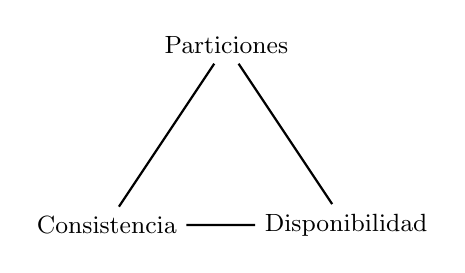
\begin{tikzpicture}[scale=0.95,every node/.style={font=\small}]
            \node (C) at (0,0) {Consistencia};
            \node (A) at (3.2,0) {Disponibilidad};
            \node (P) at (1.6,2.4) {Particiones};
            \draw[thick] (C)--(A)--(P)--(C);
        \end{tikzpicture}
    \end{center}
\end{frame}

\begin{frame}{Errores conceptuales frecuentes}
    \begin{itemize}
        \item Creer que timeout implica crash;
        \item creer que la red es confiable salvo casos extremos;
        \item asumir una visión global perfecta del sistema;
        \item tratar CAP como slogan y no como restricción bajo partición.
        \item ¿Algún otro?
    \end{itemize}
\end{frame}

\begin{frame}{Cierre}
\begin{block}{Idea final}
El pensamiento distribuido consiste en decidir correctamente bajo incertidumbre.
\end{block}

\pause

No se trata de encontrar una solución perfecta, sino de:
\begin{itemize}
\item Explicitar supuestos;
\item elegir garantías;
\item y defender el trade-off que se acepta.
\end{itemize}
\end{frame}

\end{document}
